% Sångtext till VN:s sångbok 2010.

% Denna fil kan användas som sådan, bara verserna,
% namnen och annan rådata behöver bytas ur fälten.
% Tecknet "%" markerar en kommentar som helt och 
% hållet ignoreras av programmet som läser filen.

\beginsong{Sista punschvisan}[ 		% Börja sången här
	by={},					% Författare
	sr={Auld Lang Syne},					% Melodi
	index={När punschen småningom är slut}, % Alternativa
	index={Så slickar vi, så slickar vi}]						% sångnamn
	

\beginverse*						% Börja vers
När punschen småningom är slut
och vår flaska blivit tom.
Då vänder vi den upp och ner
till dess inget rinner ur.
\endverse							% Sluta vers

\beginchorus						% Börja refräng
:,: Så slickar vi, så slickar vi
båd' utanpå och i,
och finns det ändå något kvar
får det va' till sämre dar. :,:
\endchorus

\endsong							% Sluta sång

\begin{figure}[!b]
 \begin{center}
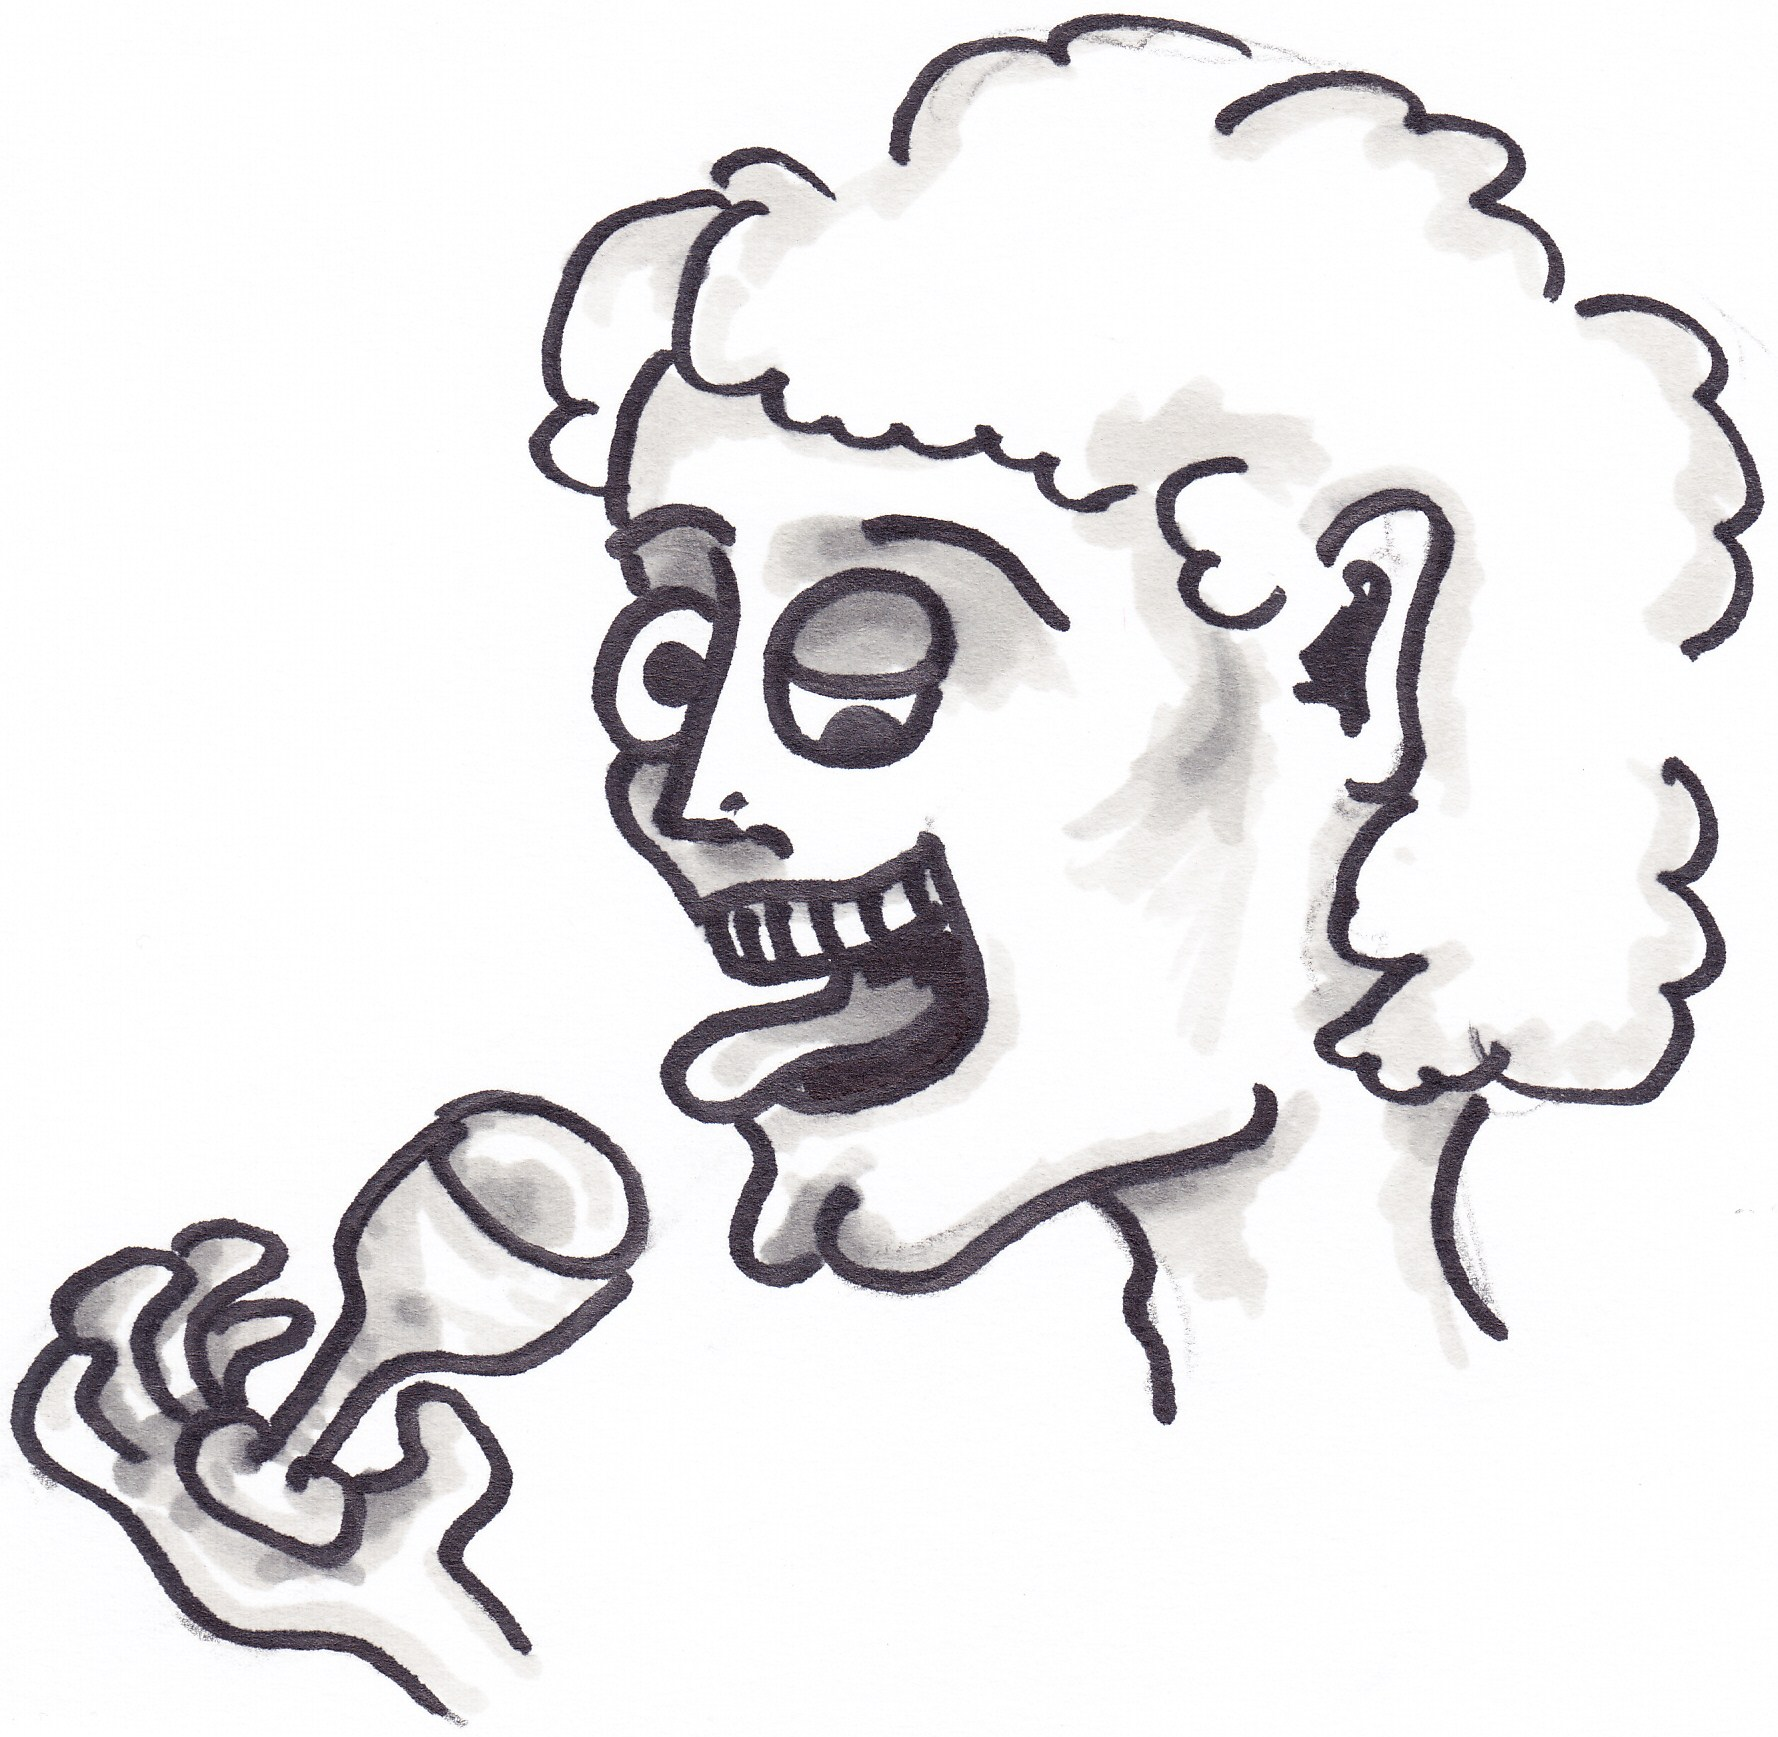
\includegraphics[scale=.3]{../bilder/sistapunschvisan.jpg} 
\end{center}
\end{figure}